\documentclass[12pt]{article}
\usepackage{graphicx}
\usepackage[
pdftex,
backref,
pagebackref,
bookmarks=true,
colorlinks=true,
linkcolor=black,
citecolor=darkgreen,
filecolor=black,
pagecolor=blue,
urlcolor=blue,
plainpages=false,
pdfpagelabels,
]{hyperref}
\usepackage{fullpage}

% %\topmargin -2.0cm
% \oddsidemargin 0in
% \evensidemargin 0in
% %\footheight 0.0pt
% \headheight 2\baselineskip
% \textwidth 6.5in
% \textheight 9.0in


%\raggedright

\begin{document}
  
\title{Description of the XDA/XDR mesh format used in libMesh}
\author{Benjamin S. Kirk, John W. Peterson, David J. Knezevic \\
        \texttt{libmesh-devel@lists.sourceforge.net} \\
	$$Revision$$} 
\maketitle

\section{Background}
The XDA and XDR formats used by libMesh to store mesh data are an extension to the mesh format used by the research code MGF, which was developed in the CFDLab at the university of Texas at Austin.  This efficient format has simply been extended to support general element types.

\subsection{XDR}
XDR, or the External Data Representation, is a standard developed by Sun Microsystems for storing binary data in a machine-independent format.  Anyone who has suffered through endian-issues in a heterogeneous machine environment will immediately see the benefit of such a format.  XDR is a C API that is available on all modern UNIX-type systems.  The XDR API is usually defined in the header file $<$rpc/rpc.h$>$.

\subsection{XDA}
So, I said XDR is available on all modern UNIX systems\ldots Unfortunately, the world has other types of machines, and not all of them immediately understand XDR.  In libMesh, an ``XDA'' file is the ASCII version of the data that would otherwise be written to an XDR file.  Another important use of the XDA file format is for debugging purposes.  If there is some problem with the data files you are writing, it is often solved by writing an ASCII version of the same data, and examining it visually for errors.  Once you've found the problem and made your changes, you can seamlessly return to writing the binary XDR format.

\section{The File Format}
libMesh mesh files consist of two sections, the header and the data.  The header contains important size information.  It defines the number of elements, number of nodes, etc\ldots that are in the mesh.  The data section contains the actual element connectivity, the nodal coordinates, and any boundary condition information.  The XDA mesh used in this example corresponds to the \texttt{reference\_elements/2D/one\_quad.xda} file distributed with libMesh.

\subsection{Header}
The header of an XDR/XDA file looks something like this:
\small
\begin{verbatim}
  LIBM 0
  1        # Num. Elements
  4        # Num. Nodes
  6        # Length of connectivity vector
  4        # Num. Boundary Conds.
  65536    # String Size (ignore)
  1        # Num. Element Types.
  5        # Element types in each block.
  1        # Num. of elements in each block at each refinement level.
  Id String
  Title String
\end{verbatim}
\normalsize
The header defines several important sizes that are used to enable efficient, block-reading of the data section. A line-by-line description of the header follows:

The first line of the file is a string that defines what code wrote the file. There are three possibilies: MGF, DEAL and LIBM. The reason for this first line is backwards-compatibility. In this document we will mostly discuss the ``LIBM'' format. This is the newest and most flexible of the three formats; it allows hybrid meshes and adaptive mesh refinement information to be written out. The number following the string "LIBM" on the first line indicates the number of levels of refinement in the mesh. The mesh in the above example has no refinement structure, so this number is zero.

The next line contains a single integer that defines the number of elements in the mesh.  Anything after the \# is ignored and may be used as a comment.

The next line contains the length of the connectivity array which is the array that contains all the data in the connectivity section of the XDA file, discussed below. This size is important since it allows us to read in the entire connectivity array for the mesh into a buffer of this length.

The number of boundary condition describes just that.  In libMesh boundary conditions are assigned to specific faces of elements.  The format for specifying boundary conditions will be discussed in the data section. We only specify boundary conditions for level 0 elements (i.e. elements with no parents). From the level 0 elements we can infer the boundary information of all other elements in the mesh.

The next line defines the maximum string size for the subsequent identification strings \texttt{Id~String} and \texttt{Title~String}. This is used to prevent buffer-overruns when reading ridiculously long titles (I think).  It may safely be ignored.  These strings may be used for identification purposes.

\subsubsection{Augmented Header}
The three lines after the string size are not read in for the MGF format, since these lines are related only to hybrid meshes (the MGF format does not support hybrid meshes).

When reading and writing meshes, libMesh orders the elements into contiguous blocks based on refinement level and element type.  For instance, consider a mesh with two levels of refinement (i.e. level 0 elements and level 1 elements) and with both quadrilaterals and triangles. First, elements are grouped according to their refinement level, so all the level 0 elements are written first, followed by the level 1 elements. Within each block of elements at a given level, they are written in blocks based on element type. So the level 0 triangles will be grouped together, as will the level 0 quadrilaterals. In this case since the mesh contains both quadrilaterals and triangles, the ``number of element types'' line in the header would be 2.  For the \texttt{one\_quad.xda} example, there is only one element type.

The reason for grouping elements in the way described above is efficiency.  It would be possible to write the elements in any order, but then two additional IDs would be necessary to define the element type and its refinement level.  Writing the elements in blocks like this allows a savings of \texttt{2*n\_elem} integers, or $2*4*$\texttt{n\_elem} bytes. Also, it makes sense to write out the elements in order of increasing refinement level because when we read in an XDA file and reconstruct the refinement hierarchy, we need to build the level 0 elements first, followed by the level 1 elements and so forth.

The next line defines the element types that the mesh contains.  The value here corresponds to the integer representation of the \texttt{enum} \texttt{ElemTypes}.  Valid values of this \texttt{enum} may be found \href{http://libmesh.sourceforge.net/doxygen/namespacelibMeshEnums.html#a145}{on the documentation page}.

The final line defines the number of elements in each block of elements of the same type at each level. This line
should contain (Number of levels) $\times$ (Number of element types) entries, 
and the sum of these values should be the number of elements in the mesh 
(defined in the second line of the header).

\subsection{Data}
The data section for this example is as follows:
\small
\begin{verbatim}
  0 1 2 3 0 -1
  0. 0. 0. 
  1. 0. 0.
  1. 1. 0.
  0. 1. 0.
  
  0 0 0
  0 1 1
  0 2 2
  0 3 3
\end{verbatim}
\normalsize

The data section consists of two mandatory and one optional section.  The mandatory sections are the element connectivity and the nodal locations.  The optional section defines the boundary conditions (note that if the number of boundary conditions is set to 0 in the header then the boundary condition section will not be read).

\subsubsection{Connectivity}
The connectivity section has two roles: (i) to define which nodes are connected to which elements, and (ii) to define the refinement hierarchy by specifying element and parent IDs.

Each element has its own line in this section. Suppose a given element has $N$ nodes, then the first $N$ entries on that element's line specify which nodes the element is connected to, and the last two entries specify the element's ID and its parent's ID respectively. In this case there is only one element, so the connectivity section contains only one line.  For this example the local nodes on the first element map to the global nodes 0, 1, 2, and 3. The element has an ID of 0, and it has no parent (it is a level 0 element) so its parent ID is -1.  More complicated example meshes may be found in the Appendix.

Unlike many unstructured mesh formats, libMesh stores the element connectivity first.  The reason for this is that, for parallel meshes, libMesh partitions on \emph{elements}.  That is to say, each element ``belongs'' to one \emph{and only one} processor.  By storing the element connectivity first elements may be distributed to various processors before the nodal locations are read.  When the nodes are read they are only sent to the processors that need them.

\subsubsection{Nodes}
The next section simply consists of $(x,y,z)$ triples defining the location of each node.  There are as many lines in this section as there are nodes defined in the header.  Note that libMesh \emph{always} expects 3 coordinate values for each point, even when the library is compiled to support only 2D meshes. The entire node array is thus $3*$\texttt{n\_nodes} entries long.  In this example the $z$ coordinate is identically 0.  In general, $z$ can be any number since it will be ignored in 2D mode.

For the XDR binary format the coordinates are treated as libMesh \texttt{real} numbers, which are defined at compile-time to be either \texttt{float}s or \texttt{double}s.  \textbf{Note:} In the future, nodes may be written as \texttt{float}s and then cast to \texttt{real}s for space savings.  In other words, don't rely on double precision for your nodal coordinates.

\subsubsection{Boundary Conditions}
Each boundary condition is defined by three integer numbers:  the element number, the side number on that element, and the boundary condition number.  There will be a line in this section for each boundary condition, up to the number of boundary conditions specified.  The boundary condition number may be any value which fits in a \texttt{short int}. As mentioned above, in a mesh with refinement hierarchy boundary conditions are only stored on for the level 0 elements. A non-level 0 element obtains boundary information from its level 0 ancestor.

Note that the boundary condition numbers mean nothing to libMesh, they are simply specified for certain faces of certain elements.  The \href{http://libmesh.sourceforge.net/doxygen/classBoundaryInfo.html}{\texttt{BoundaryInfo}} class may be used to access the boundary condition numbers assigned to a particular element face.  The user may use these boundary conditions in their code to impose boundary conditions.  There are no ``automatic'' boundary conditions in libMesh, that is there are no special boundary condition IDs that may be specified such that a certain boundary condition is imposed.  Since libMesh is a framework rather than a simulation tool it leaves the responsibility of assigning boundary conditions with the user.

\clearpage
\appendix
\section{Hybrid Mesh}
This is an example XDA hybrid-element mesh.
\small
\begin{verbatim}
  LIBM 0
  10     # Num. Elements
  11     # Num. Nodes
  52     # Length of conectivity array
  0      # Num. Boundary Conds.
  65536  # String Size (ignore)
  2      # Num. Element Blocks.
  5 3    # Element types in each block.
  2 8    # Num. of elements in each block at each level.
  Id String
  Title String
  0 4 8 7 0 -1 
  8 5 2 6 1 -1 
  7 9 3 2 -1 
  3 9 6 3 -1 
  6 9 8 4 -1 
  8 9 7 5 -1 
  4 10 8 6 -1 
  8 10 5 7 -1 
  5 10 1 8 -1 
  1 10 4 9 -1 

  0. 0. 0.
  2. 0. 0.
  2. 2. 0.
  0. 2. 0.
  1. 0. 0.
  2. 1. 0.
  1. 2. 0.
  0. 1. 0.
  1. 1. 0.
  .5 1.5 0.
  1.5 .5 0.
\end{verbatim}
\normalsize

\clearpage
\begin{figure}
  \centerline{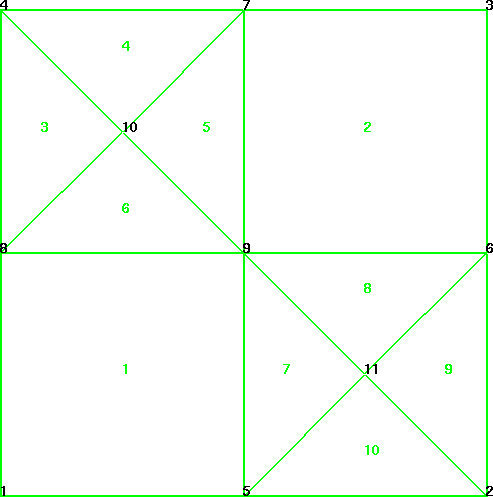
\includegraphics[width=.9\textwidth]{hybrid_mesh}}
  \caption{Hybrid element mesh (note that the numbers are off by one).}
\end{figure}

\clearpage
\section{Refined Hybrid Mesh}
Here the hybrid mesh from above has been uniformly refined once. The corresponding XDA file is:
\small
\begin{verbatim}
LIBM 1
50       # Num. Elements
33       # Num. Nodes
260      # Sum of Element Weights
0        # Num. Boundary Conds.
65536    # String Size (ignore)
2        # Num. Element Blocks.
5 3      # Element types in each block.
2 8 8 32 # Num. of elements in each block at each level.
Id String
Title String
0 1 2 3 0 -1 
2 4 5 6 1 -1 
3 7 8 2 -1 
8 7 6 3 -1 
6 7 2 4 -1 
2 7 3 5 -1 
1 9 2 6 -1 
2 9 4 7 -1 
4 9 10 8 -1 
10 9 1 9 -1 

0 11 12 13 10 0 
11 1 14 12 11 0 
13 12 15 3 12 0 
12 14 2 15 13 0 
2 16 17 18 14 1 
16 4 19 17 15 1 
18 17 20 6 16 1 
17 19 5 20 17 1 
3 21 22 18 2 
21 7 23 19 2 
22 23 8 20 2 
21 23 22 21 2 
8 23 24 22 3 
23 7 25 23 3 
24 25 6 24 3 
23 25 24 25 3 
6 25 18 26 4 
25 7 26 27 4 
18 26 2 28 4 
25 26 18 29 4 
2 26 15 30 5 
26 7 21 31 5 
15 21 3 32 5 
26 21 15 33 5 
1 27 14 34 6 
27 9 28 35 6 
14 28 2 36 6 
27 28 14 37 6 
2 28 16 38 7 
28 9 29 39 7 
16 29 4 40 7 
28 29 16 41 7 
4 29 30 42 8 
29 9 31 43 8 
30 31 10 44 8 
29 31 30 45 8 
10 31 32 46 9 
31 9 27 47 9 
32 27 1 48 9 
31 27 32 49 9 

0.000000e+00 	0.000000e+00 	0.000000e+00 	
1.000000e+00 	0.000000e+00 	0.000000e+00 	
1.000000e+00 	1.000000e+00 	0.000000e+00 	
0.000000e+00 	1.000000e+00 	0.000000e+00 	
2.000000e+00 	1.000000e+00 	0.000000e+00 	
2.000000e+00 	2.000000e+00 	0.000000e+00 	
1.000000e+00 	2.000000e+00 	0.000000e+00 	
5.000000e-01 	1.500000e+00 	0.000000e+00 	
0.000000e+00 	2.000000e+00 	0.000000e+00 	
1.500000e+00 	5.000000e-01 	0.000000e+00 	
2.000000e+00 	0.000000e+00 	0.000000e+00 	
5.000000e-01 	0.000000e+00 	0.000000e+00 	
5.000000e-01 	5.000000e-01 	0.000000e+00 	
0.000000e+00 	5.000000e-01 	0.000000e+00 	
1.000000e+00 	5.000000e-01 	0.000000e+00 	
5.000000e-01 	1.000000e+00 	0.000000e+00 	
1.500000e+00 	1.000000e+00 	0.000000e+00 	
1.500000e+00 	1.500000e+00 	0.000000e+00 	
1.000000e+00 	1.500000e+00 	0.000000e+00 	
2.000000e+00 	1.500000e+00 	0.000000e+00 	
1.500000e+00 	2.000000e+00 	0.000000e+00 	
2.500000e-01 	1.250000e+00 	0.000000e+00 	
0.000000e+00 	1.500000e+00 	0.000000e+00 	
2.500000e-01 	1.750000e+00 	0.000000e+00 	
5.000000e-01 	2.000000e+00 	0.000000e+00 	
7.500000e-01 	1.750000e+00 	0.000000e+00 	
7.500000e-01 	1.250000e+00 	0.000000e+00 	
1.250000e+00 	2.500000e-01 	0.000000e+00 	
1.250000e+00 	7.500000e-01 	0.000000e+00 	
1.750000e+00 	7.500000e-01 	0.000000e+00 	
2.000000e+00 	5.000000e-01 	0.000000e+00 	
1.750000e+00 	2.500000e-01 	0.000000e+00 	
1.500000e+00 	0.000000e+00 	0.000000e+00 	

\end{verbatim}
\normalsize

\clearpage
\begin{figure}
  \centerline{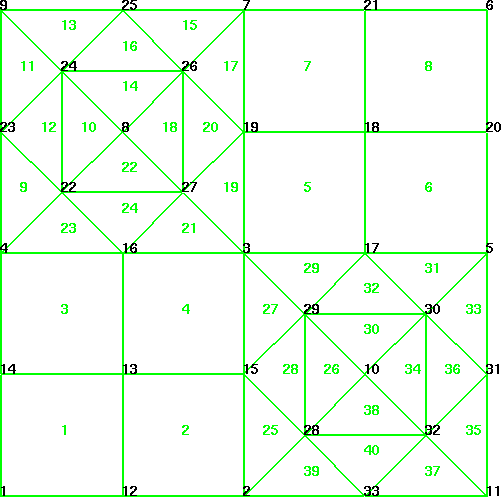
\includegraphics[width=.9\textwidth]{refined_hybrid_mesh}}
  \caption{Uniform refinement of previous hybrid mesh.}
\end{figure}


\end{document}
